\title{Basic Lessons on High School Math Olympiad Part 0} 
\date{\today}
\author{Azzam L. H. (Instagram: azzam\_29\_12)}
\maketitle
\renewcommand*\contentsname{Daftar Isi}
\tableofcontents
 
\section{Tips-tips}
	\begin{enumerate}
	    \item Latihan yang rajin dan \textbf{konsisten} setiap hari walaupun hanya 15-30 menit.
	    \item Matematika itu ilmu menulis, catat, coba-coba, dan corat-coret. Anda malas menulis dan hanya mau membaca saja? Buang-buang waktu aja.
	    \item Tidak perlu belajar materi pelajaran matematika sekolah dulu (kecuali yang dibutuhkan di olimpiade), langsung latihan soal olimpiade saja. Kemampuan matematis Anda di pelajaran sekolah akan meningkat sejalan dengan kemampuan matematika olimpiade Anda.
	    \item Kuasailah Bahasa Inggris (terutama Bahasa Inggris untuk matematika) agar anda bisa mempelajari materi-materi luar negeri dan mengerjakan soal-soal kontes luar Indonesia yang (sayangnya) masih jauh lebih bagus dari materi dan soal-soal di Indonesia.
	    \item Rajin-rajin latihan soal dari \href{https://artofproblemsolving.com/community}{Art of Problem Solving - AOPS} (\href{https://artofproblemsolving.com/community}{https://artofproblemsolving.com/community}).
	    \item Usaha tanpa doa = tidak berkah. Ada tangan tak terlihat yang membantu Anda untuk mengerti semua hal di dunia ini.

	\end{enumerate}
	
\section{Common Math Mistakes}

\begin{enumerate}
    \item $\dfrac{n}{0} \neq \infty$ tetapi \textbf{seharusnya} $\dfrac{n}{0} = \text{tak terdefinisi}$ dimana $n \neq 0$.\\
    Kecuali kalau pakai limit, baru benar, yaitu $\lim_{x \rightarrow 0^+} \dfrac{n}{x} = \infty$ dan $\lim_{x \rightarrow 0^-} \dfrac{n}{x} = -\infty$
    \item Seharusnya $\dfrac{0}{0} = \textbf{tak tentu}$.
    \item $\pi$ (\textbf{pi}) itu \textbf{dibaca "PI"} bukan dibaca "FI". 
    \item Kalau $\varphi$ (\textbf{phi}) baru dibaca \textbf{"FI"}.
    \item $\sqrt{x} \ge 0$ dengan $x \ge 0$. Jadi, hasil dari $\sqrt{(-x)^2}=|x|$ jadinya $\sqrt{(-2)^2}=2$.
\end{enumerate}
\section{Logika Dasar}
\begin{enumerate}
    \item $A \land B$ dibaca $A$ dan $B$.
    \item $A \lor B$ dibaca $A$ atau $B$.
    \item $A \equiv B$ dibaca $A$ ekuivalen $B$ (untuk logika).
    \item $\exists x$ dibaca ada $x$ atau terdapat $x$.
    \item $\forall x$ dibaca untuk semua $x$.
    \item $A \implies B$ dibaca
    \begin{enumerate}
        \item $A$ hanya jika $B$,
        \item $B$ jika $A$,
        \item $A$ mengimplikasikan $B$,
        \item $A$ menyebabkan $B$,
        \item jika $A$ maka $B$.
    \end{enumerate}
    \item $A \Longleftarrow B$ dibaca $A$ jika $B$ (kebalikannya $\implies$).
    \item $A \iff B$ dibaca $A$ jika dan hanya jika $B$. Definisinya adalah $A \iff B \equiv (A \implies B) \land (A \Longleftarrow B)$.
\end{enumerate}
Apa bedanya $A \implies B$ dan $A \iff B$? Kalau $A \implies B$ berarti agar pernyataan benar haruslah $B$ benar, $A$ bisa salah atau benar. Kalau $A \iff B$, agar pernyataan benar, haruslah $A$ dan $B$ sama-sama benar atau sama-sama salah. Contohnya:
\begin{itemize}
    \item Jika sekarang hujan, maka saya tidak pergi. (Baik sekarang hujan ataupun tidak hujan, bisa saja saya tidak pergi, jadi tidak pengaruh).
    \item Saya laki-laki jika dan hanya jika saya bukan perempuan.
        \item Saya tidak bernafas selamanya jika dan hanya jika saya tidak hidup.
\end{itemize}
\section{Himpunan}
Hanya review, harusnya sejak SMP sudah paham mengenai himpunan / \textit{set} :).

Misalkan $A$ dan $B$ adalah dua himpunan.
\begin{enumerate}
    \item $\phi$ atau $\{\}$ adalah himpunan kosong atau himpunan yang tidak mempunyai elemen.
    \item Banyak elemen dari $A$ dinotasikan dengan $|A|$ (dibaca "kardinalitas dari $A$") atau $n(A)$ .
    \item $x \in A$ dibaca $x$ elemen dari $A$.
    \item $A \subseteq B$ dibaca $A$ subset dari $B$ atau $A$ himpunan bagian dari $B$.
    \item $A \subset B$ dibaca $A$ adalah proper subset dari $B$. Bedanya dengan $\subseteq$?\\
    $\subset$ itu mirip $<$ dimana tidak mungkin $A \subset A$, tetapi $\subseteq$ itu mirip $\le$ karena mungkin $A \subseteq A$.
    \item $A \cup B$ dibaca $A$ union $B$ atau $A$ gabung $B$.
    \item $A \cap B$ dibaca $A$ intersection $B$ atau $A$ irisan $B$.
    \item $A^c$ atau $A'$ dibaca $A$ komplemen.
    \item $|A \cup B| = |A|+|B|-|A \cap B|$.
\end{enumerate}
	
\subsection{Himpunan Bilangan-bilangan}
\begin{figure}[h]
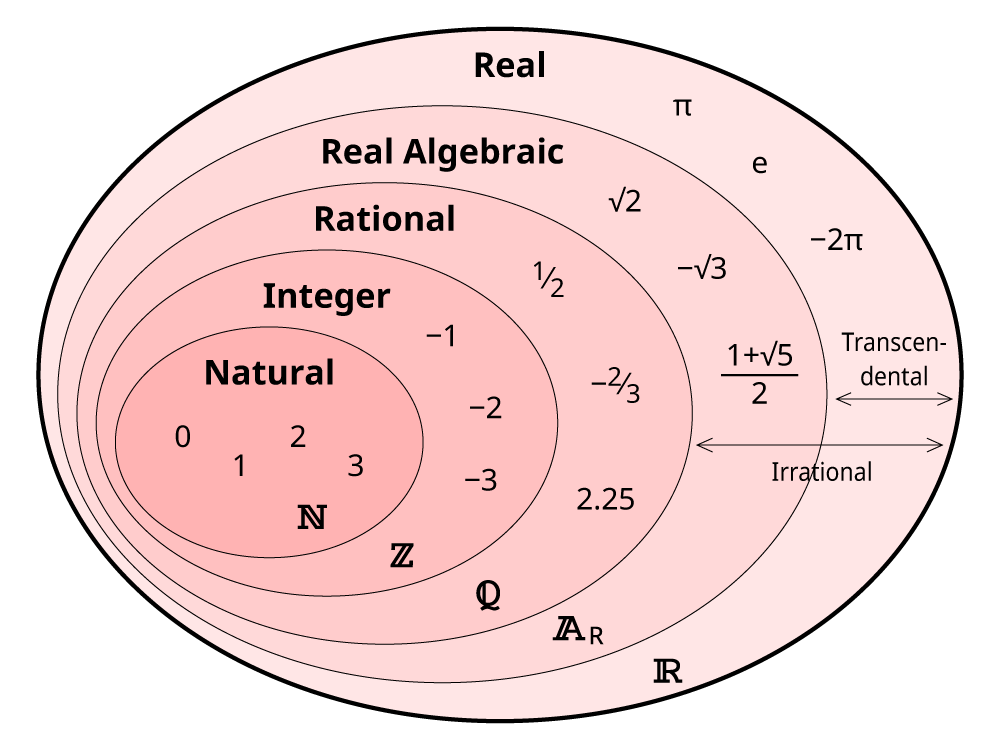
\includegraphics[width=\textwidth/2]{assets/numbers set.png}
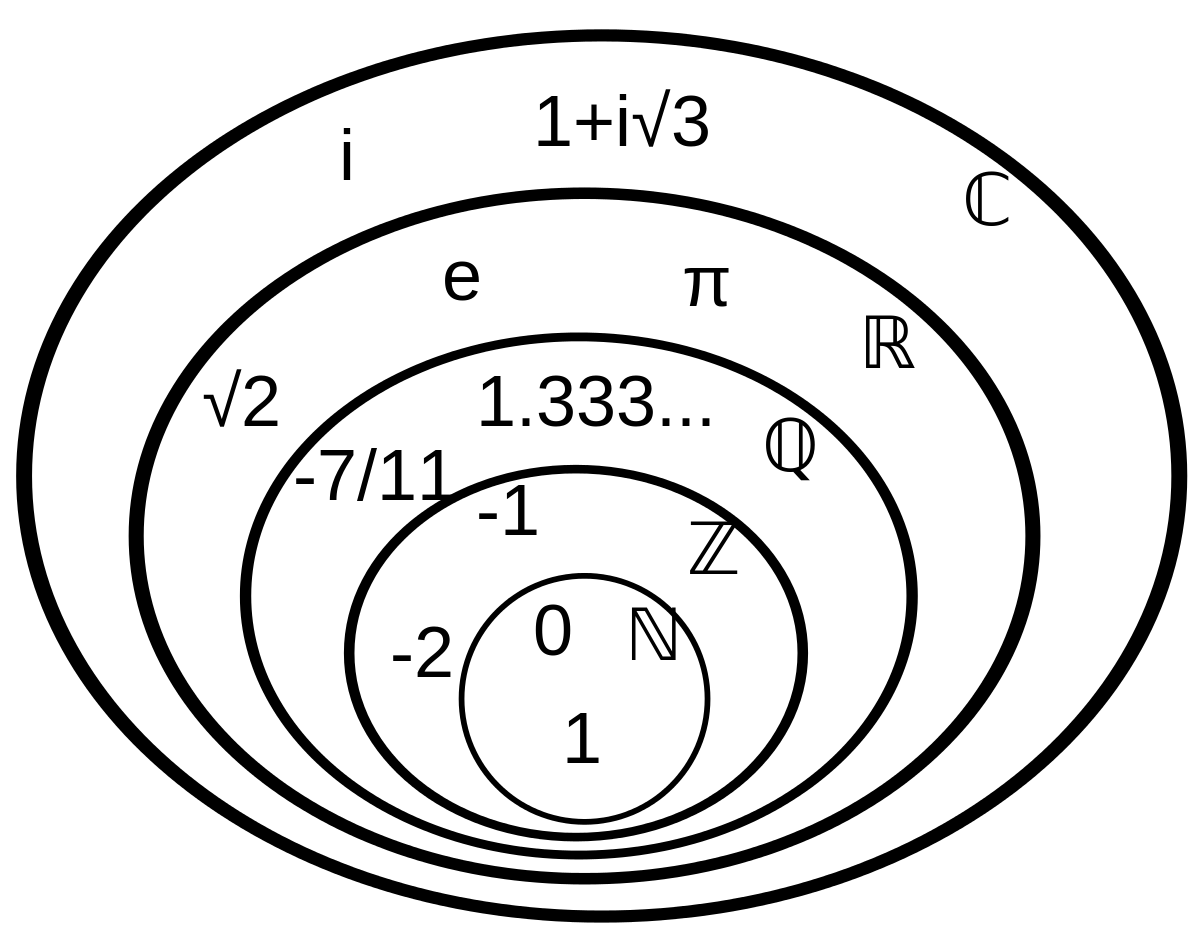
\includegraphics[width=\textwidth/2]{assets/compset.png}
\caption{dari: https://thinkzone.wlonk.com/Numbers/RealSet\_w1000.png}
\caption{dan https://en.wikipedia.org/wiki/Number}
\end{figure}

\begin{enumerate}
\item $\NN$ adalah himpunan bilangan asli (Natural Numbers) $\{1,2,3,\dots\}$. Di beberapa negara Eropa dan beberapa negara lain, himpunan bilangan asli adalah $\{0,1,2,\dots\}$.
\item $\ZZ$ adalah himpunan bilangan bulat $\ZZ=\{\dots,-2,-1,0,1,2,\dots\}$.
\item $\QQ$ adalah himpunan bilangan rasional, dengan definisi $\QQ=\{\dfrac{a}{b}\mid a\in \ZZ, b\in\ZZ^+\}$.
\item $\RR$ adalah himpunan bilangan real, semua bilangan yang ada di dunia nyata, termasuk bilangan irasional seperti $\sqrt{2}$ dan rasional.
\item $\CC$ adalah himpunan bilangan kompleks dengan definisi\\ $\CC = \{a+bi \mid a,b \in \RR \text{ dan }i=\sqrt{-1}\}$.
\item Definisikan pula $\ZZ^+$ sebagai himpunan bialangan bulat positif. Aturan yang sama juga berlaku: $\RR^+, \QQ^+$.
\end{enumerate}

